\chapter{Asking A Billionaire Lawyer How To Make \$1{,}000{,}000!}

This School of Hard Knocks interview, curated here for the LazyEarn track by LazyingArt LLC, is not a board lecture in the usual sense. Its mathematics is the arithmetic of commercial scale: how a personal-injury firm aligns incentives, converts attention into cases, converts cases into verdicts and settlements, and then protects the resulting capital from ruin. The interview itself opens twice, first as spectacle and then as explanation, and we will preserve that order. The question is not merely how rich John Morgan became; it is how a law practice was turned into a machine.

\section{A Rare Billionaire Route Through Law}

The tape begins with a teaser montage: billionaire status, large annual income, hard edges in business, and a closing life-principle question. Then the host resets and gives the real frame. The route matters. Morgan is presented not simply as a wealthy Floridian but as someone who reached billionaire scale through law, which the host treats as rare enough to count on fewer than two hands.

That is already a useful opening move. Before we ask for tactics, we are told why the case is unusual. Morgan identifies his core business plainly: personal injury law, and not just a practice, but what he claims is the largest PI law firm in North America. The interview is then allowed to do what it does best: move from spectacle to mechanism. The early question about money is there to establish scale, but the deeper question is how such scale is organized.

In the later and more precise statement, Morgan says that the firm did roughly \$2 billion in fees in a single year. We will treat that as the canonical annual fee figure for this lecture:
\begin{equation}
F \approx \$2 \times 10^9.
\end{equation}
That number is not yet an explanation. It is only a marker. The explanatory work begins when the host asks the first genuinely structural question: what single decision allowed a multibillion-dollar law firm to grow?

\section{Delegation, Partners, and the First Scale Law}

Morgan's first answer is strikingly simple: delegate, find partners one can trust, and share the business with them. This is the first law of scale in the interview. The founder does not scale by stretching himself thinner; he scales by building a system in which able people participate in the upside.

A compact way to record the economic idea is
\begin{equation}
\Pi_{\mathrm{firm}} = \Pi_{\mathrm{founder}} + \sum_{i=1}^{n}\Pi_i,
\end{equation}
where \(\Pi_{\mathrm{firm}}\) denotes total firm profit and the \(\Pi_i\) denote the participating upside of trusted partners. This equation is not an accounting identity taken from the firm's books. It is a transcript-derived schematic of Morgan's phrase that good people must make money \emph{with} the founder, not merely \emph{for} him.

\begin{definition}
A \emph{send-delete} person is someone to whom a founder can send a task once, trust the execution, and then remove the task from active attention. In the lecture's own operational shorthand, we may write
\begin{equation}
\text{send} \to \text{trust} \to \text{delete}.
\end{equation}
\end{definition}

This is more than a hiring preference. It is a criterion for reducing managerial friction. A machine whose founder must repeatedly reopen every task has not really delegated anything. A machine built from send-delete people begins to acquire the one thing that scale requires: attention that can move forward instead of recycling backward.

\section{Pain, Purpose, and Entrepreneurial Selection}

The interview does not remain in abstract management for long. After the rule of delegation comes the reason Morgan became a lawyer at all. His brother Tim was paralyzed in an accident while Morgan was in college. Morgan says that the way his brother was treated changed his life, and the later work of the firm is described through that lens. When he sees injured clients, he says he sees Tim; the vocation is therefore not only commercial but reparative.

This part of the interview matters because it prevents the chapter from becoming a sterile growth memo. Morgan does not describe his field as a neutral market opportunity discovered from nowhere. He describes pain turned into passion and purpose. In these notes, that point should remain close to the earlier scaling doctrine: the machine has a motive before it has a method.

From there the lecture widens into a claim about entrepreneurial disposition. Morgan repeatedly returns to the idea that not everybody is built for entrepreneurship. The ``paperboy'' becomes his emblem of the early hustler: daily repetition, no vacation, and the formation of commercial stamina before adulthood. The later lion-and-sloth image is harsher, but its function is the same. He is not arguing that incentives do not matter; he is arguing that incentives alone cannot create the temperament of relentless work.

The chapter should preserve the sharpness of this turn. The interview moves from injury and vocation to a broader theory of selection: some people are drawn toward difficult, repetitive, low-glamour commercial labor before they ever know what industry they will end up in. That is the human substrate onto which the later equations of scale are written.

\section{Fees, Negotiation, and the Contingent Path}

The next pivot is practical. The host asks what advice Morgan would give to a law student who wants to build something empire-sized. Morgan's answer immediately contrasts two business models: hourly billing and contingency fees. He rejects the billable-hour model not because it is illegitimate, but because, in his words, the upside is too small for the game he wants to play.

A cautious reconstruction of the contrast is
\begin{equation}
F_{\mathrm{hourly}} = r h,
\end{equation}
where \(r\) is an hourly rate and \(h\) is billable time, while contingency-fee practice is modeled by
\begin{equation}
F_{\mathrm{cont}} =
\begin{cases}
\alpha R, & \text{if the case is won},\\[4pt]
0, & \text{if the case is lost},
\end{cases}
\end{equation}
where \(R\) is the client's recovery and \(\alpha\) is the contingency fraction.

\subsection{Question \& Answer}

\paragraph{Question.} Why does Morgan think hourly billing is the wrong game if one wants empire-scale upside?

\paragraph{Answer.} Because hourly billing grows linearly with time, while contingency practice ties compensation to the magnitude of successful recoveries. In schematic form, once a case is won we obtain
\begin{equation}
\frac{F_{\mathrm{cont}}}{F_{\mathrm{hourly}}}
= \frac{\alpha R}{r h}.
\end{equation}
Morgan's point is not that every contingency case dominates every hourly matter. It is that the business model of the firm is built to participate in outcomes, not merely in labor time. If the firm is genuinely good at winning large recoveries, the upside is structurally different.

Negotiation then enters by a short aphorism: the first speaker loses. The note we should take is not that silence is magical, but that listening is informative. To size up a deal and size up a person, one must first allow information to appear. In this interview, negotiation is therefore not a theatrical trick but a discipline of withholding premature commitment.

The section then widens again into Morgan's philosophy of luck. He says that life consists of many left turns, right turns, and U-turns, and that a single different turn could have made everything different. The mathematical content here is modest but useful: he is thinking in terms of path dependence rather than deterministic self-authorship. A schematic version is
\begin{equation}
\omega = (d_1,d_2,\dots,d_n), \qquad d_k \in \{\text{left},\text{right},\text{U-turn}\},
\end{equation}
with the lecture's central claim expressed by
\begin{equation}
d_k \mapsto d_k' \quad \Longrightarrow \quad O(\omega') \neq O(\omega),
\end{equation}
where \(O(\omega)\) denotes the terminal outcome generated by the path \(\omega\). This is not a theorem from probability theory. It is the interview's way of insisting that success should be read with humility.

Faith and reputation complete the block. Morgan says he prays every night, and the best advice from a mentor is to keep one's word. Once luck enters the lecture, reputation becomes even more important: if the path contains contingency, then one of the few durable assets still under direct control is the credibility of one's promises.

\section{Reputation, Betrayal, and Error Absorption}

The lecture then darkens. The host asks what happens when one is wronged in business. Morgan's answer is not sentimental. Sometimes, he says, one pays people to walk away. He borrows a Bezos-style formulation and turns it into a surgical metaphor: identify the cancers in the business and excise them.

The key point is operational. Scale is not preserved only by adding revenue; it is preserved by removing corrosive sources of negative energy. The interview insists that positivity here is not mood management but commercial hygiene. A bad internal node can absorb more managerial attention than a weak market.

Morgan then gives a notable description of error handling inside a large firm. Lawyers make mistakes; cases can be damaged. His account is that the right response is direct disclosure to the client, coupled with the firm's malpractice insurance and financial capacity to absorb the consequences. In shorthand, the sequence is
\begin{equation}
\text{mistake} \to \text{disclosure} \to \text{insurance} \to \text{repair}.
\end{equation}
Again, this is a transcript-derived compression, not a formal legal workflow. But it captures the interview's structure: do not hide the error, do not pretend it did not happen, and do not let the client bear the loss alone.

At this point the video contains a host promotional interlude about proximity, mentorship, and a paid community. For our purposes, we compress it heavily. The important structural fact is only that the tape pauses and then resumes. When it resumes, the lecture moves from maintenance to competition and strategy.

\section{Competition, the Google Law Firm, and Brick-by-Brick Expansion}

Morgan returns from the interruption with a defense of competition itself. Competition, he says, makes people better. The comparison to Michael Jordan is not analytically deep, but it prepares the strategic theorem of the second half of the interview: ``What would Google do if it was a law firm?''

That question reorganizes the chapter. Instead of asking how a traditional law office grows, Morgan asks what a universal-access platform would look like if translated into legal service. The components are clear enough to formalize:
\begin{equation}
\mathcal{C} = N_{\mathrm{states}} \times H_{\mathrm{service}} \times \tau_{\mathrm{intake}}^{-1},
\end{equation}
with
\begin{equation}
N_{\mathrm{states}} = 50, \qquad H_{\mathrm{service}} = 24/7, \qquad \tau_{\mathrm{intake}} \approx 2 \text{ min}.
\end{equation}
This is not Morgan's notation; it is a compact way of preserving his claim that the firm should be everywhere, available continually, and easy to enter.

\begin{figure}
\centering
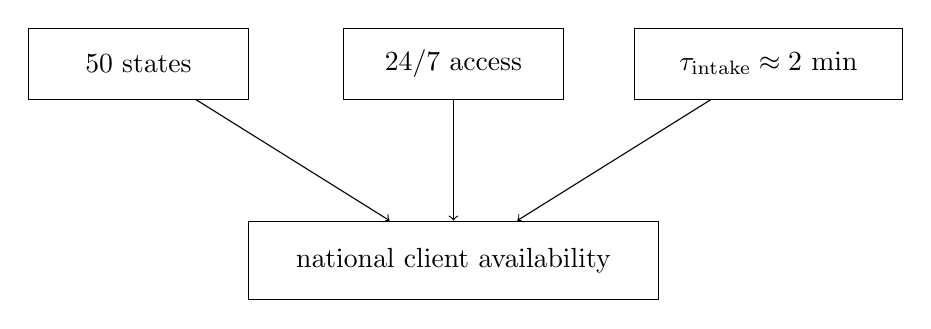
\begin{tikzpicture}[x=1cm,y=1cm]
\node[draw, rectangle, minimum width=2.8cm, minimum height=0.9cm] (a) at (-4,1.5) {\(50\) states};
\node[draw, rectangle, minimum width=2.8cm, minimum height=0.9cm] (b) at (0,1.5) {\(24/7\) access};
\node[draw, rectangle, minimum width=3.4cm, minimum height=0.9cm] (c) at (4,1.5) {\(\tau_{\mathrm{intake}} \approx 2\) min};
\node[draw, rectangle, minimum width=5.2cm, minimum height=1cm] (d) at (0,-1) {national client availability};
\draw[->] (a) -- (d);
\draw[->] (b) -- (d);
\draw[->] (c) -- (d);
\end{tikzpicture}
\caption{Transcript-derived schematic of the ``Google law firm'' idea: ubiquity, continuous access, and low-friction intake.}
\label{fig:google-law}
\end{figure}

\subsection{Question \& Answer}

\paragraph{Question.} What does it actually mean to scale a service business nationally without collapsing quality?

\paragraph{Answer.} In the lecture, it means two things at once. First, reduce access friction: broad geography, continual availability, fast intake. Second, do not confuse access with execution. Morgan's own warning later in the interview is that marketing without legal capacity makes a paper tiger. So national scale is not just more front doors. It is a larger machine whose back end can still perform.

The geography of growth is then described in a surprisingly conservative way. Morgan does not narrate a sudden leap to a national map. He says he went from Orlando to Tampa, from Orlando to Jacksonville, and from Orlando to Naples, brick by brick. The metaphor of the three little pigs is not decorative. It says that durable expansion is local, adjacent, and hurricane-resistant.

\begin{figure}
\centering
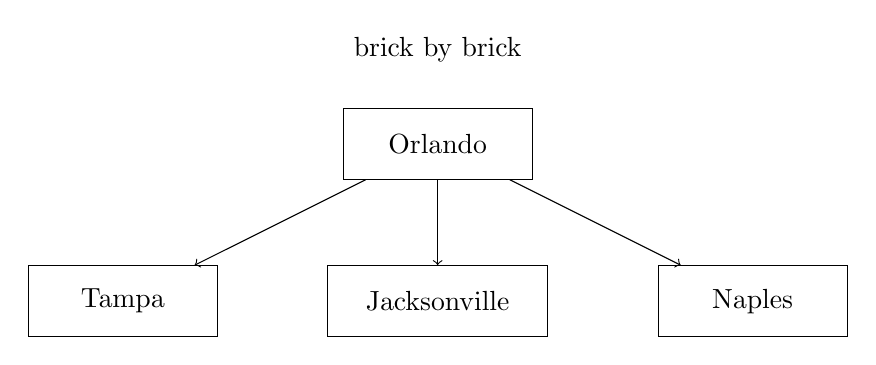
\begin{tikzpicture}[x=1cm,y=1cm]
\node[draw, rectangle, minimum width=2.4cm, minimum height=0.9cm] (o) at (0,0) {Orlando};
\node[draw, rectangle, minimum width=2.4cm, minimum height=0.9cm] (t) at (-4,-2) {Tampa};
\node[draw, rectangle, minimum width=2.8cm, minimum height=0.9cm] (j) at (0,-2) {Jacksonville};
\node[draw, rectangle, minimum width=2.4cm, minimum height=0.9cm] (n) at (4,-2) {Naples};
\draw[->] (o) -- (t);
\draw[->] (o) -- (j);
\draw[->] (o) -- (n);
\node at (0,1.2) {brick by brick};
\end{tikzpicture}
\caption{Transcript-derived schematic of adjacent-market expansion from Orlando outward.}
\label{fig:brick-scale}
\end{figure}

\section{Keeping Money: Black Swans, No Debt, and the Revenue Machine}

Having explained how the machine grows, the interview turns to a second problem: how the resulting money is kept. Morgan's formulation is compact and severe. It is hard to make money; it is harder to keep money. Losses, he says, occur when greed takes over and one enters situations that already smell wrong.

This is followed by a sequence of practical maxims: if it is too good to be true, it is too good to be true; grow or die; the best time to plant a tree was twenty years ago, and the next best time is today. These are not equations, but they are time-structure claims. They point away from regret and toward compounding action.

Morgan's asset-allocation remarks are more precise. He recommends index funds for equities, tax-free bonds yielding about \(4\%\) to \(4.5\%\), U.S.\ Treasuries, and self-investment into operating assets such as attractions, hotels, shopping centers, and apartments. He adds a hard rule for the investment bucket: once the money goes in, he does not touch it. In clean schematic form,
\begin{equation}
K_{t+1}^{\mathrm{invest}} = (1+r_t)K_t^{\mathrm{invest}},
\qquad
D_t^{\mathrm{invest}} = 0,
\end{equation}
where \(K_t^{\mathrm{invest}}\) is long-term investment capital, \(r_t\) its return rate, and \(D_t^{\mathrm{invest}}\) the withdrawal stream. The lecture does not present the rule this symbolically; the symbols simply preserve the point that permanent capital should compound rather than be repeatedly cannibalized.

The book that Morgan names as most important is \emph{The Black Swan}. His reading of it is practical rather than literary: be prepared. In the interview, preparedness immediately means cash and no debt. We may compress the doctrine as
\begin{equation}
\mathcal{P} = (\text{cash reserves},\, L=0,\, \text{readiness for shock}),
\end{equation}
with \(L\) denoting leverage. The musical-chairs metaphor that follows says the same thing in another register. When the music stops, one either has a chair or does not. In solvency language,
\begin{equation}
\text{liquidity}(t^\*) < \text{obligations}(t^\*) \quad \Longrightarrow \quad \text{failure at shock time } t^\*.
\end{equation}

\subsection{A Worked Advertising Example}

The lecture now turns to the most concrete arithmetic in the chapter. Morgan says the firm spends about \$400 million per year on advertising, while generating about \$5 billion in settlements and verdicts and about \$2 billion in fees. Using his own figures, we obtain
\begin{align}
A &\approx \$4 \times 10^8, &
S &\approx \$5 \times 10^9, &
F &\approx \$2 \times 10^9.
\end{align}
From these,
\begin{align}
\frac{A}{S}
&=
\frac{\$4 \times 10^8}{\$5 \times 10^9}
=
0.08,\\[4pt]
\frac{A}{F}
&=
\frac{\$4 \times 10^8}{\$2 \times 10^9}
=
0.20.
\end{align}

Two cautions are essential. First, \(S\) and \(F\) are not the same quantity: \(S\) is client recoveries, while \(F\) is firm fees. Second, the arithmetic alone does not prove causation. The lecture's own answer is more structural. Advertising works only because the firm can also try cases, win verdicts, and force the insurance industry to take it seriously.

That is why Morgan divides the business into two stages: ``catching fish'' and ``cooking fish.'' The first is marketing and case acquisition. The second is legal execution. We may write the mechanism schematically as
\begin{equation}
\text{marketing} \to \text{cases acquired} \to \text{verdict / settlement capacity} \to F.
\end{equation}

\begin{figure}
\centering
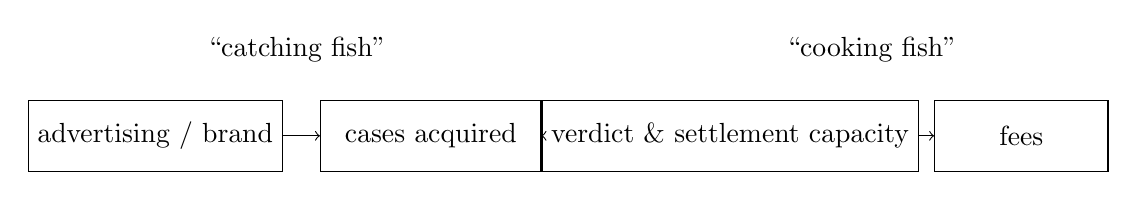
\begin{tikzpicture}[x=1cm,y=1cm]
\node[draw, rectangle, minimum width=2.8cm, minimum height=0.9cm] (m) at (-5,0) {advertising / brand};
\node[draw, rectangle, minimum width=2.8cm, minimum height=0.9cm] (c) at (-1.5,0) {cases acquired};
\node[draw, rectangle, minimum width=3.6cm, minimum height=0.9cm] (v) at (2.3,0) {verdict \& settlement capacity};
\node[draw, rectangle, minimum width=2.2cm, minimum height=0.9cm] (f) at (6,0) {fees};
\draw[->] (m) -- (c);
\draw[->] (c) -- (v);
\draw[->] (v) -- (f);
\node at (-3.2,1.1) {``catching fish''};
\node at (4.1,1.1) {``cooking fish''};
\end{tikzpicture}
\caption{Transcript-derived schematic of the two-stage revenue machine.}
\label{fig:fish}
\end{figure}

The quantitative scale of the back end is also given explicitly:
\begin{equation}
D_{\mathrm{week}} \approx 200 \text{ dockets per week}.
\end{equation}
That number explains the seriousness of the later brand claim. The brand is not merely a recognizable name. It is backed by a large litigation engine. Hence Morgan's remark that many firms may attract cases, but without trial capacity they remain paper tigers.

The interview closes by braiding this operational argument back into brand and ethics. One must make the creative creative; one must be willing to be memorable rather than interchangeable. But the long-horizon asset underneath the creative is trust. People want a winner, Morgan says, because they want to win. The lecture then ends where it began to turn serious: the golden rule, karma, and the lesson of \emph{Give and Take}. The giver, on this account, is not a sentimental figure. The giver is a long-horizon commercial actor whose reputation compounds.

\section{Summary}

The chapter's machine can now be stated compactly. First, scale comes from delegated trust and shared upside rather than founder overextension. Second, the firm's economics depend on contingent participation in outcomes rather than the simple sale of hours. Third, national reach is conceived as low-friction availability, but only works when paired with real legal execution. Fourth, wealth is preserved by resisting greed, avoiding leverage, and holding permanent capital for the long run. Finally, the machine does not end in arithmetic alone. It closes, as the interview closes, on trust, reciprocity, and the insistence that durable commercial power is inseparable from the way one treats other people.